En los capítulos previos se han utilizado funciones en diversas oprtunidades. Instrucciones como len(), range(), round(), y otras son funciones predefinidas mientras que otras deben importarse de módulos antes de ser utilizadas como \textit{sin} y \textit{cos} del módulo \textit{math}.\\

Una función debe llevar a cabo una sola tarea de forma eficiente y en caso necesario recibir los parámetros que necesite para cumplir su objetivo y devolver el resultado. Es mala práctica solicitar datos dentro de una función o confundir la devolución de los datos con la impresión del resultado en algún medio externo como la pantalla.\\

Las funciones no solo vienen definidas por librerías, el programador puede crear sus propias funciones que le permitan resolver un problema una vez y utilizar esa solución n cantidad de veces.

\section{Uso de las funciones}

Al llamar a una función (también se le dice activar o invocar) se le pasan cero o más parámetros separados por comas y encerrados entre paréntesis. Una función puede devolver un valor o no devolver nada. En caso de que no se especifique un valor de retorno, la función devuelve \textbf{None}, equivalente a \textbf{Null} de otros lenguajes.\\

\begin{pyglist} [language=python]
>>> round(14.56678, 2)
14.57
>>> round(14.56678)
15.0
>>> from math import cos
>>> cos(90)
-0.4480736161291701
>>> 
\end{pyglist}

Si una función devuelve un resultado, este es de un tipo determinado por lo que al utilizar funciones al programar se debe tener cuidado en operarlo de acuerdo a su tipo.\\

\begin{pyglist} [language=python]
>>> 1 + abs(-10)
11
>>> 3*cos(14)+123
123.4102116546235
>>> range(20,30,1+1)
[20, 22, 24, 26, 28]
>>> 12 + str(3)
Traceback (most recent call last):
  File "<stdin>", line 1, in <module>
TypeError: unsupported operand type(s) for +: 'int' and 'str'
>>> 
\end{pyglist}


\section{Definición de funciones}

Para definir una función se sigue la siguiente sintaxis:\\

\begin{pyglist} [language=python]
#!/usr/bin/python
# -*- coding: utf-8 -*-

def cuadrado(x):
    """Esta es una funcion que calcula el cuadrado"""
    return x ** 2

def suma(x, y):
    return x + y

print cuadrado(4)
print suma(5, 6)
\end{pyglist}

La línea que empieza con \textbf{def} es la cabecera de la función y el fragmento de programa que contiene los cálculos que debe efectuar la función se denomina cuerpo de la función. El valor que se pasa a una función cuando es invocada se denomina parámetro o argumento. Las porciones de un programa que no son cuerpo de funciones forman parte del programa principal: son las sentencias que se ejecutarán cuando el programa entre en acción. El cuerpo de las funciones sólo se ejecutará si se producen las correspondientes llamadas.\footnote{\cite{Marzal2003} p. 212}\\

Los nombres de las funciones deben ser únicos, no solo con respecto a otras funciones sino también a los nombres de las variables. En una función se pueden escribir todo tipo de programas, incluyendo bucles, condicionales, llamadas a otras funciones entre otras.\\

Si se desea saber si una persona es menor o mayor de edad, se puede utilizar la siguiente función:\\

\begin{pyglist} [language=python]
#!/usr/bin/python
# -*- coding: utf-8 -*-

def es_mayor_de_edad(edad):
    if edad < 18:
        resultado = False
    else:
        resultado = True
    return resultado
    
print es_mayor_de_edad(16)
\end{pyglist}

Un problema más complejo es escribir una función que responda si un número dado es o no \textit{perfecto}. Se dice que un número es perfecto si es igual a la suma de todos sus divisores excluído él mismo. Por ejemplo, 28 es un número perfecto, pues sus divisores(excepto él mismo) son 1, 2, 4, 7 y 14, que suman 28.\\

\begin{pyglist} [language=python]
#!/usr/bin/python
# -*- coding: utf-8 -*-

def es_perfecto(n):
    sumatorio = 0
    
    for i in range(1, n):
        if n % i == 0:
            sumatorio += i

    if sumatorio == n:
        return True
    else:
        return False

print es_perfecto(28)
print es_perfecto(18)
\end{pyglist}

Además de números se pueden pasar listas o cadenas como argumentos, en el siguiente ejemplo se suman todos los elementos de una lista:\\

\begin{pyglist} [language=python]
def sumatorio(lista):
    s=0
    for numero in lista:
        s += numero
    return s

print sumatorio([1,2,3,4,6])
\end{pyglist}

Debido a que en Python todo nombre de variable es tan solo un apuntador a un objeto, en Python se pueden asignar funciones con el operador =, tal como se haría con una variable.\\

\begin{pyglist} [language=python]
>>> def funcion():
...     print "Soy una funcion"
... 
>>> funcion()
Soy una funcion
>>> x = funcion
>>> x()
Soy una funcion
>>> 
\end{pyglist}

Por último, en Python, al no ser un lenguaje tipado, se pueden aplicar las mismas operaciones a diferentes tipos de datos, por ejemplo una función que sume dos parámetros puede hacer esa operación con números, listas, cadenas y en general cualquier conjunto de objetos que soporten esa operación.


\subsection{Parámetros}

Las funciones pueden tener varios parámetros y parámetros por defecto, por ejemplo:\\

\begin{pyglist} [language=python]
#!/usr/bin/python
# -*- coding: utf-8 -*-

def area_rectangulo(altura, anchura=10):
    return altura * anchura 
    
print area_rectangulo(3, 4)
print area_rectangulo(3)
print area_rectangulo(anchura=5, altura=6)
\end{pyglist}

Se puede ver que se pueden pasar los parámetros en cualquier orden, mencionando en forma explícita el nombre de cada uno.

\subsubsection{Parámetros arbitrarios}

Una función puede recibir 'n' cantidad de parámetros, donde n es un número desconocido de argumentos. Estos argumentos llegaran a la función en forma de tupla. Para definir los parámetros arbitrarios, se coloca el nombre de la tupla precedida por un asterisco (*).\\

\begin{pyglist} [language=python]
# -*- coding: utf-8 -*-

def n_parametros(param1, *n_params):
    print "Parametro 1 es: ", param1

    print "Parametros arbitrarios: ", n_params
        
print n_parametros(100, "Hola", 200, True, [1,2,3])
\end{pyglist}

También se pueden recibir parámetros arbitrarios como pares de clave=valor, en este caso el nombre del parámetro debe estar precedido por dos asteriscos (**).\\

\begin{pyglist} [language=python]
# -*- coding: utf-8 -*-

def n_parametros(param1, *n_params, **dict_params):
    print "Parametro 1 es: ", param1

    for param in n_params:
        print param

    # Los argumentos arbitrarios tipo clave, se recorren como diccionarios
    for clave in dict_params:
        print "El valor de la clave ", clave, " es ", dict_params[clave]


n_parametros(100, "Hola", 200, True, [1,2,3], val1="valor 1",
                   val2="valor 2", num1=123)
\end{pyglist}


\subsubsection{Parámetros empaquetados}

El caso contrario al anterior es una función que espera una lista fija de parámetros y solo recibe una lista de valores. En este caso un asterisco (*) debe preceder al nombre de la lista o tupla pasada como parámetro. \\

\begin{pyglist} [language=python]
def calcular(importe, descuento):
    return importe - (importe * descuento / 100)

datos = [1500, 10]
print calcular(*datos)

datos = [1500]
print calcular(100, *datos)
\end{pyglist}

En caso se pase un diccionario, el parámetro debe estar precedido por dos asteriscos (**).

\begin{pyglist} [language=python]
def calcular(importe, descuento):
    return importe - (importe * descuento / 100)
    
datos = {"descuento": 10, "importe": 1500}
print calcular(**datos)
\end{pyglist}

\section{Parámetros por valor y referencia}

\begin{quotation}
En el paso por referencia lo que se pasa como argumento es una referencia o puntero a la variable, es decir, la dirección de memoria en la que se encuentra el contenido de la variable, y no el contenido en si. En el paso por valor, por el contrario, lo que se pasa como argumento es el valor que contenía la variable.\\

La diferencia entre ambos estriba en que en el paso por valor los cambios que se hagan sobre el parámetro no se ven fuera de la función, dado que los argumentos de la función son variables locales a la función que contienen los valores indicados por las variables que se
pasaron como argumento. Es decir, en realidad lo que se le pasa a la función son copias de los valores y no las variables en si.\\

Si quisiéramos modificar el valor de uno de los argumentos y que estos cambios se reflejaran fuera de la función tendríamos que pasar el parámetro por referencia.\\

En C los argumentos de las funciones se pasan por valor, aunque se puede simular el paso por referencia usando punteros. En Java también se usa paso por valor, aunque para las variables que son objetos lo que se hace es pasar por valor la referencia al objeto, por lo que en realidad parece paso por referencia.\\

En Python también se utiliza el paso por valor de referencias a objetos, como en Java, aunque en el caso de Python, a diferencia de Java, todo es un objeto (para ser exactos lo que ocurre en realidad es que al objeto se le asigna otra etiqueta o nombre en el espacio de nombres local de la función).\\

Sin embargo no todos los cambios que hagamos a los parámetros dentro de una función Python se reflejarán fuera de esta, ya que hay que tener en cuenta que en Python existen objetos inmutables, como las tuplas, por lo que si intentáramos modificar una tupla pasada como parámetro lo que ocurriría en realidad es que se crearía una nueva instancia, por lo que los cambios no se verían fuera de la función.\\

(...)\\

\textbf{En resumen: los valores mutables se comportan como paso por referencia, y los inmutables como paso por valor.}
\end{quotation} \footnote{\cite{Duque} p. 40}\\

Si no se desea modificar un objeto mutable pasado como parámetro, se puede pasar una copia de este a la función o copiarlo dentro de la función, de tal manera que nunca sea modificado.\\

\begin{pyglist} [language=python]
L = [1, 2]
changer(X, L[:])

def changer(a, b):
    b = b[:]        # Copy input list so we don't impact caller
    a = 2
    b[0] = 'spam'   # Changes our list copy only
\end{pyglist}


\section{Variables locales y globales}

En el cuerpo de las funciones se pueden definir y utilizar variables, las cuáles no son iguales a las variables que se crean en el cuerpo principal del programa. Cuando se define una variable dentro de una función, esta variable no puede ser utilizada fuera de la función ya que no existe fuera del ámbito donde fue creada.\\

Las variables que solo existen en el cuerpo de la función se llaman \textit{variables locales} y las que existen en el cuerpo del programa son llamadas variables globales. También los parámetros de una función son considerados variables locales. al acabar la ejecución de una función, todas sus variables locales dejan de existir.\\

Las variables globales, a diferencia de las locales son accesibles desde cualquier parte del código, incluyendo una función, excepto si dentro de la función hay una variable con el mismo nombre, en cuyo caso se utiliza la variable local y no la variable global.

\begin{pyglist} [language=python]
#!/usr/bin/python
# -*- coding: utf-8 -*-

cad = 'cad1'
c = 'cadena2'

def imprime_saludo(saludo):
    cad = saludo
    print cad, c

def prueba(f):
    f('Jelou')

prueba(imprime_saludo)
print cad
\end{pyglist}

Si se referencia una variable global desde una función, esta es utilizada, pero si se le asigna un valor, la variable es local si relación con la variable global del mismo nombre.

\begin{pyglist} [language=python]
>>> def func():
...     print x
... 
>>> x = 10
>>> func()
10

>>> def func2():
...     x = 10
...     print x
... 
>>> x = 30
>>> func2()
10
>>> 
\end{pyglist}


Si se desea modificar una variable global dentro de una función se utiliza la palabra \textbf{global}, que es lo más parecido a una declaración que se puede encontrar en Python, con la diferencia que no es una declaración de tipo o tamaño sino de \textbf{namespace}.\\

\begin{pyglist} [language=python]
>>> def func():
...     global x
...     x = 34
... 
>>> x = 10
>>> func()
>>> x
34
>>>
\end{pyglist}

Aún cuando la variable no hubiera sido utilizada fuera de la función, al declararla con global pasa a estar en el ámbito global del módulo en que se ejecuta.


\section{Buenas prácticas con funciones}

\begin{itemize}
\item La función debe ser en lo posible independiente del exterior. Utilizar argumentos y devolver valores es con frecuencia la mejor manera de mantener la modularidad de la función.

\item Solo usar variables globales cuando sea necesario.

\item No cambiar los parámetros mutables a menos que eso sea explícito en la funcionalidad del método.

\item Una función debe tener una y sola una funcionalidad.

\item En lo posible una función debe ser pequeña. Keep it simple and short.
\end{itemize}


\section{Módulos}

Al escribir funciones se simplifican los programas, y no solo se simplifican sino que además esa función puede ser utilizados en otros programas, como en el siguiente ejemplo:\\

\begin{pyglist} [language=python]
#!/usr/bin/python
# -*- coding: utf-8 -*-

def area_rectangulo(altura, anchura):
    return altura * anchura
\end{pyglist}

A este programa se le dará el nombre de \textit{area\_rectangulo.py} y será utilizado desde el programa \textit{calculo.py}, que es el siguiente:\\

\begin{pyglist} [language=python]
#!/usr/bin/python
# -*- coding: utf-8 -*-

from area_rectangulo import area_rectangulo

print area_rectangulo(1,4)
\end{pyglist}

Cada archivo de texto con código Python es un Módulo, los cuales proveen una forma de particionar el espacio de nombres (namespace). Todo objeto en Python ``vive'' en su respectivo módulo y para ser utilizado en otro debe ser explícitamente importado.

\subsection{Arquitectura de un programa en Python}

En un programa python, a menos que sea muy sencillo, van a existir varios archivos con código y configuraciones las cuales serán importadas por otros archivos del programa.\\

El script de mayor nivel (el primero en ser ejecutado) contiene el flujo de control del programa y utiliza el resto de módulos (archivos .py) para obtener librerías y configuraciones. A su vez cada módulo puede importar lo que necesite de otros módulos. En Python no existen tipos de archivos diferentes para programas y librerías como en otros lenguajes.\\

En la siguiente imagen se puede apreciar la arquitectura de un programa en Python. \footnote{\cite{Lutz2012} p. 672}

\begin{figure}[ht!]
   \centering
   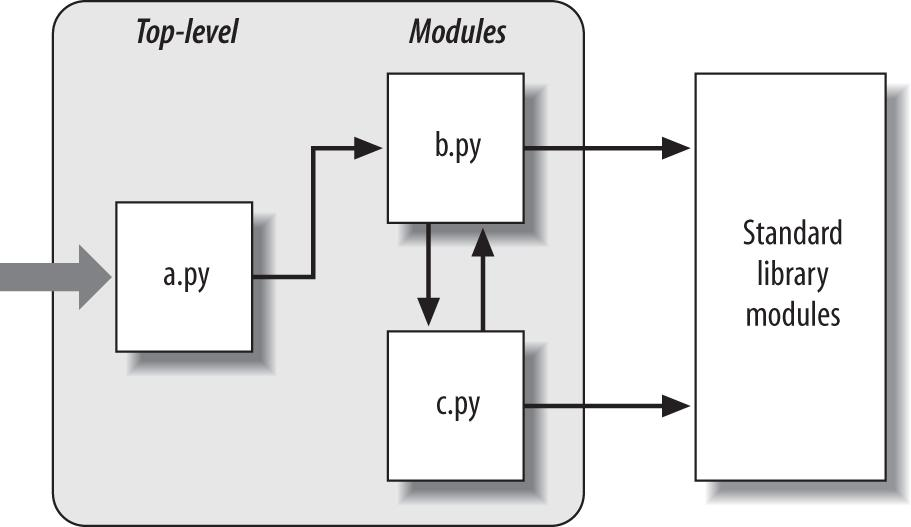
\includegraphics[scale=0.5]{imagenes/arquitectura_python.jpg}
   \caption{Arquitectura de un programa en Python}\label{graf:arquitectura-python}
\end{figure}

\newpage

\section{Ejercicios}

\begin{enumerate}
\item Escriba una función llamada raiz\_cubica que devuelva el valor de la raíz cúbica de x.

\item Escriba una función llamada area\_circulo que, a partir del radio de un círculo, devuelva el valor de su área. Utiliza el valor 3.1416 como aproximación de pi o importe el valor de pi que se encuentra en el módulo math.

\item Escriba una función que convierta grados Farenheit en grados centígrados. (Para calcular los grados centígrados se restan 32 a los grados Farenheit y se multiplica el resultado por cinco novenos.)

\item Implementa una función que reciba una lista de números y devuelva la media de dichos números. Tenga cuidado con la lista vacía (su media es cero).

\item Diseñe una función que calcule la multiplicación de todos los números que componen una lista.

\item Define una función que, dada una cadena x, devuelva otra cuyo contenido sea el resultado de concatenar 6 veces x consigo misma.

\item Escriba una función que, dada una lista de cadenas, devuelva la cadena más larga. Si dos o más cadenas miden lo mismo y son las más largas, la función devolverá una cualquiera de ellas.

\item Escriba una función que reciba dos listas y devuelva los elementos comunes a ambas, sin repetir ninguno (intersección de conjuntos).

\item Escriba una función que, dada una lista de números, devuelva otra lista que sólo incluya sus números impares.

\item Escriba una función que reciba una número indeterminado de números y devuelva el promedio.

\item Escriba una función que reciba un número indeterminado de pares clave=valor y los imprima en pantalla.
\end{enumerate}